\documentclass{bioinfo}
\usepackage[english]{babel}
\copyrightyear{2015} \pubyear{2015}
\usepackage{natbib}
\bibliographystyle{natbib.bst}


\access{Advance Access Publication Date: Day Month Year}
\appnotes{Manuscript Category}

\renewcommand{\cite}{\citep}
\usepackage{todonotes}

\begin{document}
\firstpage{1}

\subtitle{Subject Section}
\newcommand{\name}{Voodoo }

\title[short Title]{\name: Combining Bottom-up and top-down approaches through graph learning over interaction networks for drug-target-interaction prediction}
\author[Sample \textit{et~al}.]{Tilman Hinnerichs\,$^{\text{\sfb 1,}*}$ and Robert Hoehndorf\,$^{\text{\sfb 2}}$}
\address{$^{\text{\sf 1}}$Department, Institution, City, Post Code, Country and \\
$^{\text{\sf 2}}$Department, Institution, City, Post Code,
Country.}

\corresp{$^\ast$To whom correspondence should be addressed.}

\history{Received on XXXXX; revised on XXXXX; accepted on XXXXX}

\editor{Associate Editor: XXXXXXX}

\abstract{\textbf{Motivation:} Text Text Text Text Text Text Text Text Text Text Text Text Text
Text Text Text Text Text Text Text Text Text Text Text Text Text Text Text Text Text Text Text
Text Text Text Text Text Text Text Text Text Text Text Text Text Text Text Text Text Text Text
Text Text Text Text Text Text
Text Text Text Text Text.\\
\textbf{Results:} Text  Text Text Text Text Text Text Text Text Text  Text Text Text Text Text
Text Text Text Text Text Text Text Text Text Text Text Text Text  Text Text Text Text Text Text\\
\textbf{Availability:} Text  Text Text Text Text Text Text Text Text Text  Text Text Text Text
Text Text Text Text Text Text Text Text Text Text Text Text Text Text  Text\\
\textbf{Contact:} \href{tilman.hinnerichs@kaust.edu.sa}{tilman.hinnerichs@kaust.edu.sa}\\
\textbf{Supplementary information:}10264703 Supplementary data are available at \textit{Bioinformatics}
online.}

\maketitle
\section{Introduction}

\cite{Survey2018}\\
In history, traditional remedies, that were known for their medicinal
properties lead to drugs by extraction of the functional
ingredients. Alternatively, characteristics and features of potential
drugs were detected by accident like in the case of penicillin. More
recently, biological drug targets can be found \textit{in silico}
through discovery of suitable computational predictors.


The challenge of accurately predicting drug-target-interactions (DTI)
has shown its importance in the fields of drug repurposing and
repositioning, and in the exploration of novel drugs and their
interaction partners. Knowledge about those links between compounds
and their target proteins help in an array of medical and
pharmaceutical studies. Additionally, those associations can be
utilized to identify disease specific targets, leading to desirable
therapeutic effects.

With the rapidly growing field of machine learning approaches and
their application to bioscientifical problems in the realm of
bioinformatics, different kinds of data, such as long DNA sequences
could be utilized for feature generation, while rapid advances were
made. Almost all state of the art models for drug-target-interaction
prediction were based on the usage of neural networks with increasing
size.\todo{Needs ref, or reformulate}

Only recently, the technique of graph learning was introduced by
\citet{GCNConv} through graph convolution algorithms, and improved and
altered under usage of different kernels \cite{ChebConv, ARMAConv},
attention mechanisms \cite{GATConv}, random walks \cite{APPNPConv},
and mixtures of both \cite{SAGEConv}. While based on diverse systems,
they can be relevant for testing distinct hypothesis for given
graphs. While convolutional filters are suitable for finding patterns
among the the given graph, attention mechanisms are more relevant for
discovery of important regions within. Lately, graph learning
approaches found application for computing compound representations
for DTI prediction.

Approaches on this rather sophisticated\todo{Try to avoid}
problem\todo{Need to state the problem clearly here or at end of prev
  paragraph} can divided into top-down or network approaches
(\textbf{CITATION}), and bottom-up or molecular approaches
(\textbf{CITATION}). Top-down approaches take advantage of other data
such as diseases (CITATION), side effects, knowledge graphs or
ontologies, in order to learn representations for both compound and
protein. \todo[inline]{We call these approaches ``top-down'' because
  they start with the observable characteristics induced by a drug and
  infer the targets based on the likely molecular mechanisms that
  result in these phenotypes.} On the other hand, bottom-up approaches
attempt to learn from chemical properties of proteins or drugs to
infer candidate drug--target interactions. For drugs, molecular
structure (CITATION GraphDTA), molecular fingerprints, similarity to
other drugs (See Bioinf Survey), and other molecular features may be
used. On the protein side, secondary structure prediction (CITATION),
contact prediction (CITATION), or simply\todo{Don't use ``simply''.}
convolution over the amino acid sequences can be used to obtain a
feature representation for a given proteins. However, both bottom-up
and top-down approaches to drug--target interaction prediction
\todo[inline]{replace: ``contain and share some problems'' with
  something like ``have some limitations''} that are not solvable within
themselves.
\todo[inline]{Following is not sufficiently precise; here, you need to
clearly state the challenges faced by both approaches, ideally with
references.}
Thus, bottom-up approaches share the lack of ability to
generalize, which we will show in later sections, and usually focus on
engineering sophisticated features for the drugs, while neglecting to
formulate meaningful features on the protein side. Top-down approaches
lack the ability to spot small differences to cope with small
differences within the drug structure and rely heavily on given data
for the considered drug-target pair. The latter is not suitable for
predictions on novel or unseen compounds, as e.g., data on side
effects or its impact on diseases is seldom given for novel drugs.

In order to design such a feature for proteins and drugs,
respectively, we make use of the interaction networks for both
proteins and compounds. Drug-drug interaction networks were introduced
and standardized by \citet{Boyce2015} and have been used for clinical
decision support \cite{Scheife2015}. Drug-drug interaction networks
may give a hint on common targeted pathways. As an additional compound
feature we will use semantic side effect similarity, which we will
discuss later on\todo{Generally, try to avoid pointers to ``later''.}.

Protein-protein interaction networks have shown great results in $\dots$(\cite{Vazquez2003}, \cite{Ackerman2019}) in granting context for molecular system biology. However, these contexts were never applied to the problem of drug-target-interaction prediction. Thus we formalized our hypotheses over these interaction graphs and will test them in the following chapters.

\enlargethispage{12pt}

\section{Methods}
\subsection{Problem Description}
The issue of predicting drug-target interactions can be described
quite briefly: For a given drug and a given protein we want to
determine whether those interact or not.  We do not differentiate
between types of interaction such as activation and inhibition, and do
not predict the strength of the interaction.  If we additionally make
the closed world assumption, i.e., assume that our knowledge is
complete and all drug--protein pairs without a known interaction do
not interact, we can formulate the problem as a binary classification
task.


\subsection{Datasets}
The data for the different parts of this model were obtained from
various sources. Starting with the protein-protein interactions, we
fetched $\approx 11000$\todo{precise number} human proteins with over 170.000 links from
STRING \citep{STRINGv10}. For the drug-target interactions themselves,
we fetched 137.000 links from STITCH database \citep{STITCHv5}. As
both STRING and STITCH provide probability scores for each
association, we filtered them as advised by a threshold of 700, thus
only obtaining likely interactions.

For the ontology segment we utilized PhenomeNET \citep{PhenomeNET2011}, a collection of various ontologies such as Human Phenotype Ontology \citep{HPO2018}, Gene Ontology (\citet{GOoriginal2000} \citet{GOrecent2020}), Mammalian Phenotype Ontology \citep{MP2009} and numerous others. \todo{which ontologies to cite}
Side effects and their links to drugs were obtained Side Effect Resource (SIDER)\citep{SIDER} and structured according MedDRA database \citep{MedDRA}. They were mapped to PhenomeNET with aid of \textit{Phenomebrowser.net}, which provides a SPARQL query endpoint for the mentioned resources. \\

For comparative evaluation we used the gold standard dataset introduced by \citet{Yaminishi2008}, which includes both drug-target interaction pairs and side effects.\\ 
 
Eventually, we only considered proteins that had at least one link in either STITCH or STRING, and drugs with at least one side effect and one existing target. Thus, the intersection between these resources yielded 1160 drugs and 6680 human proteins for the training phase. We provide links to and methods for the necessary data in the provided Github repository.\\

\subsection{Evaluation and metrics}

\todo[inline]{First part is not about evaluation but optimization
  objectives, should go in the Model section:}
As the number of drug-targets are sparsely given w.r.t.\todo{no
  acronyms} to the number of both drugs and proteins considered, the
resulting training, validation and testing datasets are highly
imbalanced. As there are only $~22.000$\todo{exact number} links in
the considered subset the ratio
\begin{equation*}
	\frac{\#dti\_links}{\#drugs \cdot \#proteins} \approx 360,
\end{equation*}
consequently needing compensation in the computed loss function and
appropriate metrics for the evaluation.

Therefore, we weighted all positive drug-protein pair samples with
this ratio by introducing the following loss function w.r.t.\todo{no
  acronym} to binary cross-entropy:
\begin{equation}
	l(x,y) = - w \left[ y \cdot \log x + (1 - y) \cdot \log (1 - x) \right]
\end{equation}
for given prediction $x$ and target $y$. We average this loss among
all drug-protein pairs in the training set, leading to a stable
environment for the used optimizing scheme \textit{Adam}
\citep{Adam2014}. We implemented a 5-fold cross validation among the
proteins as justified in the results section. Furthermore, we used
early stopping to detect plateaus in the training process.

\todo[inline]{This needs to be more elaborate: add the micro- vs
  macro-averages here (formulas)}
To assess each model, we computed the \textit{area under receiver
  operating characteristic}-score (AUROC), \textit{F1-score} (F1) and
\textit{Matthews correlation coefficient} (MCC) for each considered
hyperparameter configuration setting.

\todo[inline]{Remove from here:}
Avoiding validation overfitting, we eventually tested the best
performing model on the Yamanishi dataset as presented and
discussed. Furthermore, we compare our results on this very dataset
with various other cutting edge approaches to DTI-prediction.


\subsection{Model}

\todo[inline]{Introduce the notion of top-down and bottom-up:}
In order to build a method that incorporates both top-down and
bottom-up features, we first created a model for each
individually. Hence, we assemble rich molecular structure based
features for drugs from
\textit{SmilesTransformer} \citep{SmilesTransformer} and proteins from
\textit{DeepGOPlus} \citep{DeepGoPlus}. \textit{SmilesTransformer}
introduces an autoencoder, learning over the SMILES strings and thus
the molecular organization of each drug in an unsupervised manner. On
the other hand, we take advantage of the pretrained models of
\textit{DeepGOPlus}, obtaining features from the proteins amino acid
sequence, showing significant performance in the field of protein
function prediction. Thus, both embeddings seem to suitably supplement
the following ontology based representations.


In the top-down section, we used \textit{DL2vec} \citep{DL2vec2020} to
obtain ontology based representations. DL2vec constructs a graph by
introducing vertices and edges for each ontology class and axiom,
respectively, followed by random walks starting from each
entity. These walks are eventually learned on using a Word2vec
\citep{Word2vec2013} model. Thus, we pick up rich, neighbourhood
focused representations for each entity, which has shown great results
for representing protein function and phenotypes. The overall
structure of the ontology can be seen in Figure~\ref{fig:Onto}.

\begin{figure}[!tpb]%figure1
	\centerline{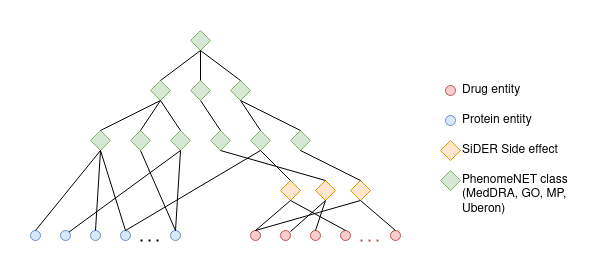
\includegraphics[width=0.5\textwidth]{figures/drug_protein_ontology_network.png}}
	\caption{Drugs and proteins with annotations to SiDER and PhenomeNET}
	\label{fig:Onto}
\end{figure}


As we wanted to learn from the similarity of drug side effects and
protein phenotypes we opted for a deep siamese network approach, hence
learning a high-dimensional embedding emphasizing this identity by
forcing a maximal cosine similarity between these embeddings. On the
other hand we built a deep neural network for the molecular structure
based features, also benefiting from the siamese network
architecture. Therefore, the precomputed embeddings are run through a
deep neural network transformation (DNNT) which also reduces the
eventual representation size for drugs and proteins separately. An
example structure for both types of features can be found in
Figure~\ref{fig:SiameseNetwork}.

\begin{figure}[!tpb]%figure1
	\centerline{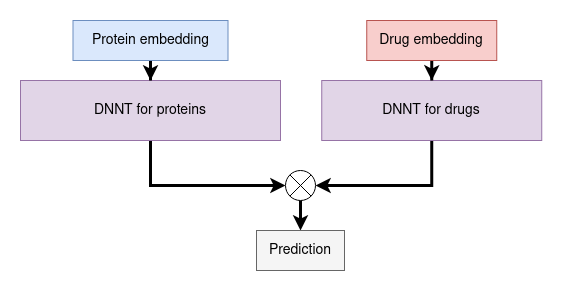
\includegraphics[width=0.35\textwidth]{figures/siamese_network.png}}
	\caption{Siamese network applied to molecular and DL2vec
          features, utilizing deep neural network transformations
          (DNNT). The similarity function $\otimes$ yields the
          similarity between both transformed embeddings e.g. by
          computing the cosine similarity.}
	\label{fig:SiameseNetwork}
\end{figure}


\subsubsection{Graph convolutional layers}
These molecular and ontology based sub-models were added to a larger
graph convolutional model, based on the protein-protein interaction
(PPI) graph. The PPI dataset is represented by a graph $G=(V,E)$,
where each protein is represented by a vertex $v\in V$, and each edge
$e\in E\subseteq V\times V$ symbolizes an interaction between two
proteins. Additionally, we introduce mapping
$x:V\rightarrow\mathbb{R}^{d}$ projecting each vertex $v$ to its node
feature $x_v = x(v)$, where $d$ denotes the dimensionality of the node
features.
 
As described before, graph convolution has shown significant
performance increase in a variety of tasks. While there are various
methods out there we will only introduce the most basic one here. A
graph convolutional layer \citet{GCNConv} consists of a
learnable weight matrix followed by an aggregation step, formalized by
\begin{equation}
	\mathbf{X}^{\prime} = \mathbf{\hat{D}}^{-1/2} \mathbf{\hat{A}}
	\mathbf{\hat{D}}^{-1/2} \mathbf{X} \mathbf{\Theta}
\end{equation}
where for a given graph $G=(V,E)$, $\hat{A} = A + I$ denotes the
adjacency matrix with added self-loops for each vertex, $D$ is
described by $\hat{D}_{ii} = \sum_{j=0} \hat{A}_{ij}$, a diagonal
matrix displaying the degree of each node, and $\Theta$ denotes the
learnable weight matrix. Added self-loops enforce that each node
representation is directly dependent on its own preceding
one. Notably, the number of graph convolutional layers stacked equals
the radius of relevant nodes for each vertex within the graph.

The update rule for each individual node is
\begin{equation}
	\mathbf{x}^{\prime}_i = \mathbf{\Theta} \sum^{N}_{j}
	\frac{1}{\sqrt{\hat{d}_j \hat{d}_i}} \mathbf{x}_j
\end{equation}
where both $\hat{d}_i, \hat{d}_j$ are dependent on the edge weights
$e_{ij}$ of the graph. With simple, single-valued edge weights such as
$e_{ij}=1 \text{ }\forall (i,j)\in E$, all $\hat{d}_i$ reduce to
$d_i$, i.e., the degree of each vertex $i$. We denote this type of
graph convolutional neural layers with \textsc{GCNConv}.


While in this initial formulation the node-wise update step is defined
by the sum over all neighbouring node representations, we are able to
alter this formulation to another message passing scheme.  We are able
to rearrange the order of activation function $\sigma$, aggregation
$\mathrm{AGG}$ and linear neural layer $\mathrm{MLP}$ with this
formulation as proposed by \citet{GENConv2020}:
\begin{equation}
	\mathbf{x}_i^{\prime} = \mathrm{MLP} \left( \mathbf{x}_i +
	\mathrm{AGG} \left( \left\{
	\mathrm{\sigma} \left( \mathbf{x}_j + \mathbf{e_{ji}} \right) +\epsilon
	: j \in \mathcal{N}(i) \right\} \right)
	\right)
\end{equation}
where we will generally only consider
$\sigma \in \{\mathrm{ReLU}, \mathrm{LeakyReLU}\}$. We will denote
this generalized layer type as \textsc{GENConv}, following the
notation of \citet{PytorchGeometric}.  While the reordering is mainly
import for numerical stability, this alteration also addresses the
vanishing gradient problem for deeper convolutional networks
\cite{GENConv2020}. Additionally, we can also generalize the
aggregation function to allow different weighting functions such as
learnable $\mathrm{SoftMax}$ or $\mathrm{Power}$ for the incoming
signals for each vertex, substituting the averaging step in
\textsc{GCNConv}. Hence, while \textsc{GCNConv} suffers from both
vanishing gradients and signal fading for large scale, highly
connected graphs, each propagation step in \textsc{GENConv} emphasizes
signals with values close to $0$ and $1$. The same convolutional
filter and weight matrix are applied to and learned for all nodes
simultaneously, and the resulting information\todo{Which information?
  Specify} hold no information on their own connectivity.

\begin{figure}[!tpb]%figure1
	\centerline{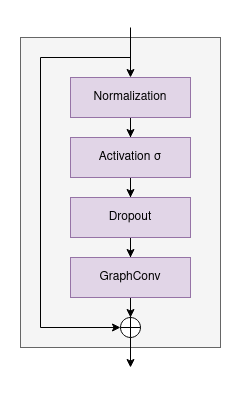
\includegraphics[width=0.5\columnwidth]{figures/ResGraphConvBlocks.png}}
	\caption{Residual architecture built by \citet{DeepGCN2019} and \citet{DeeperGCN2020} enabling deeper graph convolutional models}
	\label{fig:ResGraphConvBlocks}
\end{figure}

We employ another mechanism to avoid redundancy and fading signals in
stacked graph convolutional networks, which was introduced by
\citet{DeepGCN2019} and refined in \citet{DeeperGCN2020}. The authors
propose a residual network architecture and normalization scheme. This
structure is depicted in Figure~\ref{fig:ResGraphConvBlocks} resulting
in reusable residual blocks, which can be stacked multiple times,
thereby not losing focus of each node neighbourhood.



\subsubsection{Hyperparameter tuning}
To find the best hyperparameter configuration for the proposed model
we performed a grid search to find the most expressive and
non-redundant representation. We pretrained the bottom-up and the
top-down model separately and aimed at best performing models
w.r.t. previously described metrics. We optimized embedding sizes,
depth of the neural network, optimizer, learning rate and layer types
using an extensive, manual grid search. \todo[inline]{Specify range of
  values searched here; even better if you have the intermediate
  results and can put them here (better: in the supplement).}


\section{Results}

\subsection{Choosing a cross-validation splitting scheme}
As in machine learning inference is derived from the underlying data, models and data are naturally and intrinsically linked. Thus, the more we understand about the pitfalls and biases within the data, the more we can try to bypass these difficulties. We will hereby abbreviate, e.g., a cross validation splitting scheme as \glqq split\grqq{} determining the train, validation and test subset of a given dataset. \\
Especially within DTI prediction, one can observe elemental and basic skews \citep{Pahikkala2014}. (1.) Frequently, novel drugs are designed by altering non-functional components of a drug, leading to two and more very similar drugs, designed to target the same proteins (\textbf{CITATION?}). This bias can lead to \glqq hidden duplicates\grqq{} that can distribute among the train-test split, skewing the ultimate predictive performance. (2.) Additionally, within the realm of DTI prediction, some proteins, which we will denote as \textit{hub proteins}, have significantly more known interactions with drugs than others. In the considered subset of STITCH database, $5\%$ of the proteins had $40\%$ of the interactions, with similar biases for Yamanishi and Drugbank (\citet{Drugbank2007} and \citet{Drugbank2017}) datasets, making them easy and reliable predictors. (3.) The second distortion could be based on a publication bias for more \glqq valuable\grqq{} proteins due to their disease involvement, such as e.g., cancer, leading to more research and eventually more interacting drugs regarding those. Thus if we aim to find a drug for a given protein, the challenge is to develop a training and evaluation scheme, that does not simply overfit to those biases.\\

In general, when concerning cross-validation splitting schemes for DTI prediction, there are the following three options:
\begin{enumerate}
	\item Build split over drugs
	\item Build split over drug-target pairs
	\item Build split over proteins
\end{enumerate}
where the first and third option concern splitting drugs and proteins, respectively, into train, validation and test sets, and arranging the corresponding drug-target interactions. Hereby, different training and prediction schemes lead to divergent expressiveness of the resulting model. \\
The most common scheme for DTI prediction is the split over drug-target pairs \citep{Survey2018}, where likely all drugs and targets of the validation and testing phase have already occurred in the training phase, as part of other drug-target pairs. Thus, the first and second splitting scheme are exposed to the first dataset bias and are hence more likely vulnerable to transductive inference by just predicting recently seen structures, rather than implementing inductive inference and generalizing over the drug representations. Second, these two strategies are more susceptible to the second and third bias, as only in these cases the model may overfit on the number of existing interactions, while in the third scheme the number of interactions of the test proteins is not known. \\






Considering the publications of the last 


In general, drug-target interaction prediction is the task of accurately predicting, whether for a given drug and a given protein there is a biological interaction within the target organism. Hereby, different training and prediction schemes lead to divergent expressiveness of the resulting model. However, when building the train-test split over compound-protein pairs for building the actual model, there are the following three options:

\todo[inline]{Relate these to the issues listed above:}
\begin{enumerate}
	\item Build split over drugs
	\item Build split over drug-target pairs
	\item Build split over proteins
\end{enumerate} 
In general, recent works do perform their split over the drugs or drug-target pairs (\cite{Survey2018}, CITATION). As there are hopefully many more drugs to discover, the drug split scheme both emphasizes the drug repurposing idea, by applying unseen compounds to existing targets, but also benefits from more complicated drug representations, leading to tremendous\todo{???} results. This performance gain is based on minor variations among large groups of pharmaceuticals, that are easy to acquire\todo{evidence}. The second scheme has knowledge on all drugs and all proteins, and is thus prone to overfitting and the same development bias. Eventually, as there only limited drug-targets \citep{Overington2006}, predicting per protein is rather counter-intuitive. As it is hard to generalize over proteins representations, we aim at reaching similar performances for both drug and protein splitting schemes. \\

In general, recent works do perform their split over the drugs or drug-target pairs (\cite{Survey2018}, CITATION). The first is more relevant for novel drugs, as it is much more likely to test a new compound than a innovative protein. However, it lies in the very nature of the used datasets, making the prediction for new drugs much easier. Thus, drugs are often built by minor variations of existing drugs, thus leading to no deviations in the functional group of that very compound (CITATION/EXAMPLE). When distributed over both train and test split, the models do not perform inductive inference and generalize, but rather implement transductive inference by just predicting the recently seen structures. Hence, when entirely new molecules are seen, the models perform much worse

The same applies to splits of drug-target pairs, as all drugs were already seen, and novelty cannot be coped with.

As mentioned in the introduction it is quite difficult to learn suitable features from proteins. In general, attempts search for motifs in the protein sequences under usage of convolutional neural networks and filters, which is more suitable for tasks like protein function prediction, than for for drug-target interaction prediction, and lack a more in-depth hypothesis on the protein side, while investing in refined drug features. \\
Thus, building splitting over proteins is the most challenging of the three options. \\



\subsection{Baseline model}
Our aim is to develop and evaluate a computational model to predict
drug--target interactions. Specifically, given a protein, we are
interested in identifying the drugs that may target the protein; this
scenario is motivated by the need to identify drugs that can target a

\subsection{\name identifies drugs that target a protein}

We developed \name as a computational model to predict drug--target
interactions. Specifically, given a protein, \name will identify and
rank drugs that likely target this protein. \name combines two 
types of features: structural information for drugs and proteins that
can be used to determine if they may physically interact, and 

This scenario is motivated by the need to identify drugs that can target a
specific protein that may be associated with a disease or abnormal
phenotypes.
Our aim is further to combine two different types of features:
structural information based on protein structure and molecular drug composition, and their respective observable characteristics. \\

Before introducing the core of our eventual model, we propose a suitable naive baseline model in order to analyze and understand the existing approaches and this novel method for drug target interaction prediction. For given lists $D, P$ of drugs and proteins, respectively, and a set of known interactions $Int := \{(d_i, p_i) \}$, we construct an interaction matrix $M_{int}\in\{0,1\}^{|D|\times|P|}$ with 
\begin{equation*}
	M_{ij} = \begin{cases}
		1 & \text{if } (d_i, p_j)\in Int\\
		0 & otherwise
	\end{cases}
\end{equation*}
describing for all drug--protein whether there is a known interaction or not. We now rank all proteins $p_j\in P$ descending by their number of drug interactors, characterized by 
\begin{equation*}
	f: P \rightarrow \mathbb{N} \text{ with } f:p_j \mapsto \sum_{i=0}^{|D|}M_{ij}
\end{equation*}
by summing over the columns of $M_{ij}$ and ranking these sums.
We now finish our baseline predictor $P_k$ by predicting all drugs to interact with the top $k$ targets, denoted by $TopK(P)$ w.r.t. $M_{ij}$ from the previously introduced ranking, formalized by 

\begin{equation*}
	P_k: D\times P \rightarrow \{0,1\} \text{ with } P_k: d_i, p_j \mapsto \begin{cases}
		1 & \text{ if }p_j \in TopK(P)\\
		0 & otherwise
	\end{cases}
\end{equation*}
with the only hyperparameter $k$. Note particularly, that the consequent prediction of $P_k$ is not dependent on the considered drug $d_i$, and will thus predict all drugs similarly for a given protein $p_j$. Subsequently, this naive predictor is not yielding any valuable information on the individual interactions with drugs for a given protein. Also note the possibility for a similar predictor by calculating the top $k$ interacting drugs, respectively.

To obtain a prediction for a given drug-protein pair\todo{should this
  be about pairs, or rather something like ``given a protein, we aim
  to find a drug...''? I.e., find a consistent way to separate
  yourself language-wise from a naive prediction of pairs.}, we first
build DL2vec representations\todo{In results: talk about what they are
supposed to DO (``embeddings/representations of the phenotypes and
functions...''), not how you implement them (you could use something
else, for example).} for both drugs and proteins over PhenomeNET, while also preparing structural, molecular representations. Hence, we pretrain the siamese networks for both molecular and ontology features, yielding the deep neural network transformers for both methods and both drugs and proteins, individually. These embeddings are now added to the graph neural network as node features, where we start an end-to-end learning and training process. Notably, like in the pretraining phase, we rely on siamese neural networks, enforcing similar representations for fitting drug-protein pairs. The overall architecture can be seen in Figure~\ref{fig:Fullmodel}.

\subsection{High level description}

For a given protein, we want to find all suitable interacting drugs, \textbf{among a set of known drugs}.
To obtain a prediction for a given drug-protein pair, we first
build representations embodying both phenotypes and functions for both drugs and proteins, while also preparing structural, molecular representations, e.g., utilizing DL2vec over PhenomeNET and the prebuilt features from SMILES transformer and DeepGOPlus. Note that this approach can be easily generalized, profiting from other protein function and phenotype representation methods. \\ 
Hence, we pretrain the siamese networks for both molecular and ontology features, yielding the deep neural network transformers (DNNT) for both methods, and both drugs and proteins, individually. These embeddings are now added to the graph neural network as node features, where we start an end-to-end learning and training process. Notably, like in the pretraining phase, we rely on siamese neural networks, enforcing similar representations for fitting drug-protein pairs. The overall architecture is depicted in Figure~\ref{fig:Fullmodel}.\\

\begin{figure}[!tpb]
	\centerline{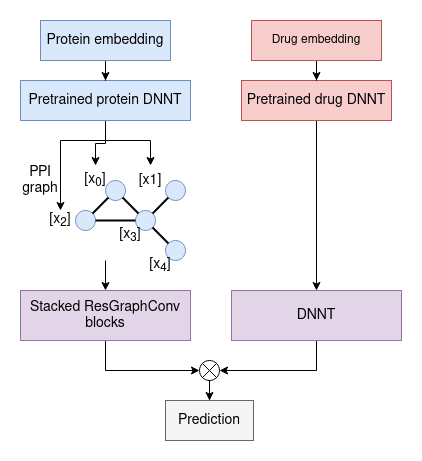
\includegraphics[width=0.45\textwidth]{figures/full_model.png}}
	\caption{Full DTI prediction model based on the pretrained deep neural network transformers (DNNT) for either molecular structure or ontology based features. The transformed protein representations are added to each corresponded protein as node features for the graph convolutional steps. }
	\label{fig:Fullmodel}
\end{figure}

Through the very nature of the graph convolutional neural network, we build the transformed representation for all proteins in every forwarding step of the model. Note particularly, that the same convolutional filter and weight matrix are applied to and learned for all nodes simultaneously. By construction, for a single drug we can compute and predict all its interactors in a single run of the model, leading to significantly less computing time. 








\section{Findings}

\subsection{Deification of our method}
\begin{itemize}
	\item we built protein function and ontology based features based on DL2vec
	\item Ontology derived protein function focused features are highly predictive for dtis
	\item We built a versatile template for various features to test localization on the PPI graph
	\item normal GCNs don't work on PPI graph, as it is highly connected $\rightarrow$ needs stronger more expressive aggregation function $\rightarrow$ GENConv in residual blocks for better numerical stability
	\item protein functions localize on the PPI graph, while molecular features don't
	\item all AUROC in \% AUROC score on STITCH
	
	\begin{tabular}{|l|r|r|}
		\hline
		DNNT model&Without graph model&With graph model\\
		\hline
		MolPred&$69$&$69$\\
		PhenomeNETPred&$88$&$92$\\
		\hline
		MolPred + PhenomeNETPred & $89$ & $93$\\
		\hline
	\end{tabular}
	\item microAUC for MolPred + PhenomeNETPred on graph is about $93+-$
	\item and on yamanishi dataset
	
	\begin{tabular}{|l|r|r|}
		\hline
		DNNT model&Without graph model&With graph model\\
		\hline
		PhenomeNETPred&$83$&$84$\\
		\hline
		MolPred + PhenomeNETPred & $83$ & $84.5$\\
		\hline
	\end{tabular}
	\item MicroAUC is about $83$
\end{itemize}

\subsection{How to insult other methods}
\begin{itemize}
	\item Only few other methods perform their split over proteins \citep{Survey2018}, DTI-CDF does it
	\item Running split over proteins is harder than, drug and drug protein pair split (see below table)
	\item this applies for both DTI prediction and drug target affinity prediction (and Saras gene-disease association)
	\item using indications is like cheating, as not applicable for searching new drugs
	\item drug indications are highly predictive for downstream tasks, but lack capability to differentiate highly related drugs/proteins
	\item Stratified Cross validation is suitable for training, but \textbf{NOT} for validating and testing (Uselessly high AUPRC)
	\item microAUC is a superior and more intuitive metric for drug repurposing $\rightarrow$ why for each protein and not for each drug
	
	\begin{tabular}{|l|p{1cm}|p{1cm}|p{1cm}|r|}
		\hline
		Approach&Splitting scheme&Original AUROC score&Protein split AUROC&MicroAUC\\
		\hline
		DTINet&DP pairs&$91$&$84.1$&$67.2$\\
		DTIGEMS+&DP pairs&$93$& $72.2$& $67.8$ \\
		DTI-CDF&Proteins&$83$&$83$&$79$\\
		\hline
	\end{tabular}
	\item A naive predictor (ranking proteins) and predict each drug similarly achieves cutting edge performance ($87.5$ AUROC for whole dataset, $85.5$ for 5-fold cross validation in drug-split) $\rightarrow$ No prot focused microAUC possible. $\rightarrow$ hub proteins
	\item Yamanishi Dataset is only partially suitable \todo{for
            comparing results}, if everybody just derives a suitable subset (DTIGEMS)
	\item This also applies to drug target affinity prediction. We were hereby able to roughly reproduce the results from MolTrans (Bioinformatics) on BioSnap

\end{itemize}

\begin{figure}[!tpb]%figure1
	\begin{tabular}{|l|p{1cm}|p{1cm}|p{1cm}|r|}
		\hline
		Approach&Splitting scheme&Original AUROC score&Protein split AUROC&MicroAUC\\
		\hline
		DeepDTI&Drugs&$87.6$&$75.9$&$70.1$\\
		DeepDTA&DP pairs&87.6&$76.7$&$69.4$\\
		DeepConv-DTI&DP pairs&88.3&$76.6$&$73.0$\\
		MolTrans&DP pairs&89.5&$77.0$&$74.0$\\
		
		\hline
	\end{tabular}
\end{figure}



\subsection{Tested hypotheses}

In this work we are testing the following hypotheses:
\begin{enumerate}
	\item Can we build a model that outperforms state of the art approaches, combining top-down and bottom-up approaches?
	\item Are interaction networks sufficient to improve the performance of simple molecular predictors?
\end{enumerate}
We will test the first hypothesis by building a model that takes both top-down and bottom-up features into account. Thus, we propose a novel approach to combine those mutual exclusive attempts, through the usage of interaction networks, similarity and molecular features. Additionally, we test the latter by building a simple molecular DTI predictor and enhance it under usage of the interaction networks.\\

For the bottom-up approach we build a model that only relies on molecular features, which we will discuss in more detail in the following methods chapter. For the combination of both approaches we now attach the predictions to the protein-protein interaction graph as node features for future graph learning steps. In this graph we tried to find both patterns and regions for each drug that could be of interest through application of different graph convolutional layers, which in return represent the feature for each protein. Representing the drug we take the drug-drug interaction graph and the semantic similarity over side effects which we will explain in the following paragraphs.

\section{Methods}

\subsection{Models}
The used model consists of two separate models, that help to fuse together the two methods:
\begin{enumerate}
	\item The molecular predictor
	\item The interaction network based predictor
\end{enumerate}
We build the molecular predictor by using pretrained, molecular fingerprints models for both drugs and proteins. Regarding proteins, we used the pretrained feature generator from \textit{DeepGoPlus} (\citep{DeepGoPlus}) that was originally designed for protein function prediction and is regarded as state of the art for this purpose. For drugs we used a pretrained fingerprint model from \textit{SMILES transformer} (\cite{SmilesTransformer}), that provides a simple and fast method to compute fingerprints through autoencoder models. The encodings from these two models were funneled into a simple deep neural network (see Figure~\ref{fig:01}) with few fully connected. \\
The results of that prediction flow into the annotation of the protein-protein interaction (PPI) graph as depicted in (IMAGE). Hereby, the predictions of the molecular predictor are used as node features for the graph, with respect to the given drug. Thus, given a compound-target pair, the nodes of the PPI graph now hold bottom-up features, which can now be processed by the graph learning algorithms. \\
The PPI graph is processed by different graph convolutional layers, that may underline the importance of either patterns or regions within the graph, to obtain a feature vector for the wanted node. In contrast to learning over whole graphs we perform node classification within the graph. These layers are either graph convolutional layers, that learn a certain kernel over the graph, or attention based. Different layers of both and other types such as were tested.  \\
The drug-drug interaction features are retrieved by choosing the corresponding row in the adjacency matrix of the graph, thus leading to quite simple features. \\
For the semantic similarity feature, that once again represents a top-down attribute, we artificially link each drug to its corresponding side effects in the MedDRA hierarchy. Concerning this hierarchy, drug-drug similarity is computed by the Resnik similarity (\cite{Resnik1995}). For the given compound we take the corresponding row of this symmetric similarity matrix. \\

Thereby, we concatenate these three features together and funnel them into another deep neural network as depicted in figure \ref{fig:02}. This network finally yields our prediction. We hereby perform splits over both drugs and proteins, in order to test and show the discrepancy and increasing difficulty.\\ Implementation was done in PyTorch (\cite{Pytorch}) and is available on Github under \href{github.com/thinnerichs/KAUST-dti-metabol}{github.com/thinnerichs/KAUST-dti-metabol}. Graph learning methods were build with help of PyTorch-Geometric (\cite{PytorchGeometric}), a geometric deep learning extension library for PyTorch, that recently got a lot of attention in the machine learning community. This library gives the potential to use many state of the art graph learning mechanisms, such as plain but effective graph convolution (\citet{GCNConv}), Chebychev kernels (\cite{ChebConv}), ARMA kernels (\cite{ARMAConv}), translation-invariant operators (\cite{FeaStConv}), attention mechanisms (\cite{GATConv}), random walks (\cite{APPNPConv}) and mixtures of the latter two (\cite{SAGEConv}). The performance of these various layer types were tested for this particular problem, as discussed in the results section.

\begin{figure}[!tpb]%figure1
	\centerline{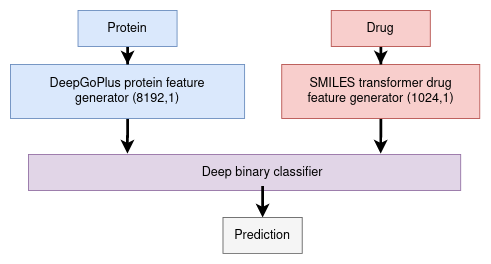
\includegraphics[width=0.4\textwidth]{figures/MolecularPredictor.png}}
	\caption{Molecular predictor based on the generated features from DeepGoPlus and SMILES transformer.}\label{fig:MolPred}
\end{figure}

\begin{figure}[!tpb]%figure2
\centerline{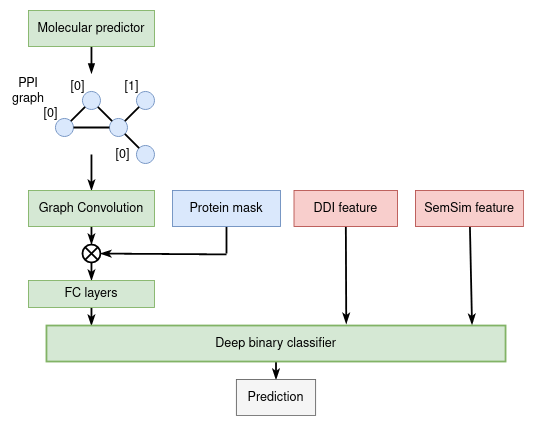
\includegraphics[width=0.4\textwidth]{figures/InteractionNetwork.png}}
\caption{Deep neural network that predicts based on drug-drug interaction features and semantic similarity features over side effects for drugs, and graph convolution over protein-protein interaction networks for proteins. Protein and drug features are represented by blue and red, respectively.}\label{fig:02}
\end{figure}

\section{Discussion}







%%%%%%%%%%%%%%%%%%%%%%%%%%%%%%%%%%%%%%%%%%%%%%%%%%%%%%%%%%%%%%%%%%%%%%%%%%%%%%%%%%%%%
%
%     please remove the " % " symbol from \centerline{\includegraphics{fig01.eps}}
%     as it may ignore the figures.
%
%%%%%%%%%%%%%%%%%%%%%%%%%%%%%%%%%%%%%%%%%%%%%%%%%%%%%%%%%%%%%%%%%%%%%%%%%%%%%%%%%%%%%%






\section{Conclusion}

\vspace*{-10pt}


\section*{Acknowledgements}

\vspace*{-12pt}

\section*{Funding}

This work has been supported by the... Text Text  Text Text.\vspace*{-12pt}

%\bibliographystyle{natbib}
%\bibliographystyle{achemnat}
%\bibliographystyle{plainnat}
%\bibliographystyle{abbrv}
%\bibliographystyle{bioinformatics}
%
%\bibliographystyle{plain}
%
\bibliography{citations}


\end{document}

%%% Local Variables:
%%% mode: latex
%%% TeX-master: t
%%% End:
